%\documentclass[11pt]{report}
\documentclass[a4paper,11pt,twoside,onecolumn,openright]{memoir}
\usepackage{geometry}
\geometry{a4paper}
%\usepackage[parfill]{parskip}%Activate to begin paragraphs with an empty line rather than an indent
\usepackage[pdftex]{graphicx}
\usepackage{amssymb}
\usepackage{epstopdf}
\usepackage{natbib}
%\usepackage{ltxfront}
\usepackage{tocvsec2}
\usepackage[hang,footnotesize,bf]{caption}
\usepackage[pdftex,bookmarks=true]{hyperref}
\usepackage{enumerate}
\bibpunct{[}{]}{;}{a}{}{,}
\DeclareGraphicsRule{.tif}{png}{.png}{`convert #1 `dirname #1`/`basename #1 .tif`.png}


%Interacting with Smartphones on Tabletop Computers
%Combining Smartphones and Tabletops: Interaction Design

\title{\Huge TIDE: Using Device Composition on Tabletop Computers to Extend the Smartphone Experience.}
\author{\textbf{Master Thesis}\\by\\Leo Sicard\\(091181-lnsi)\\
\\
\textbf{Supervisor:}\\Professor Jakob E Bardram\\
\\}
\date{March 1st, 2012\\IT University of Copenhagen, Denmark}

\begin{document}

%\maketitle
%\begin{figure}[h!]
%  \centering
%    \includegraphics[width=0.8\textwidth]{images/tide314}
%\end{figure}
%\clearpage

\pagestyle{empty}

\begin{centering}
\hfill\\
\hfill\\
\hfill\\
\hfill\\

\Huge TIDE: Using Device Composition on Tabletop Computers to Extend the Smartphone Experience.
\hfill\\
\hfill\\
\begin{figure}[h!]
  \centering
    \includegraphics[width=0.8\textwidth]{images/tide314}
\end{figure}
\large
\hfill\\
\hfill\\
\textbf{Master Thesis}\\by\\Leo Sicard\\(091181-lnsi)\\
\hfill\\
\hfill\\
\textbf{Supervisor:}\\Professor Jakob E Bardram\\
\hfill\\
\hfill\\
\hfill\\
\hfill\\
\hfill\\
\hfill\\
March 1st, 2012\\IT University of Copenhagen, Denmark\\
\end{centering}
\clearpage

\newpage
\hfill\\
\hfill\\
\hfill\\
\hfill\\
\hfill\\
\hfill\\
\hfill\\
\hfill\\
\hfill\\
\hfill\\
\hfill\\
\hfill\\
\hfill\\
\hfill\\
\hfill\\
\hfill\\
\hfill\\
\hfill\\
\hfill\\
\hfill\\
\hfill\\
\hfill\\
\hfill\\
\hfill\\
\hfill\\
\hfill\\
\hfill\\
\hfill\\
\hfill\\
\hfill\\
\hfill\\
\hfill\\
\hfill\\
\hfill\\
\hfill\\
\hfill\\
\linebreak
IT University of Copenhagen\\
Rued Langgaards Vej 7, DK-2300 K\o benhavn S, Denmark\\
Phone +45 72185000\\
itu@itu.dk\\
www.itu.dk\\
%\mbox{}
\clearpage

\hfill\\
\hfill\\
\hfill\\
\hfill\\
\hfill\\
\hfill\\
\hfill\\
\hfill\\
\hfill\\
\hfill\\

\begin{abstract}
Tabletop displays are now appearing in public spaces.
They present a horizontal interactive surface that is ideal in social situations, and they support a touch-based experience which appeals to all users.
Modern smartphones are able to support most users' daily computing tasks, and their mobility bring spontaneity to the computer interaction.
However, the screen size of smartphones is a limitation when viewing graphically intense content and in situations with multiple users.

This thesis focuses on extending the smartphone experience to tabletop displays.
It investigates the use of \emph{device composition} to allow smartphone users to spontaneously annex the display space made available by tabletops.
In particular, this report presents the design, implementation and evaluation of \emph{TIDE (Tabletop Interactive Display Extension)}: a composite device that integrates a smartphone to a tabletop by way of UI replication, with focus on \emph{spontaneous user interaction}.

The design process shows that by following a human-centered approach and using interaction techniques that are familiar to most users, the system can be designed to be easy to learn and easy to use.
The implementation of TIDE demonstrates that it is feasible to build this type of system on standard hardware and many standard platforms.
Moreover, TIDE supports multiple simultaneous smartphones, and uses computer vision to track the location of the devices on the display.
The evaluation of TIDE, in the form of a participant-based usability study, shows that the system is highly learnable, easy to use, and useful in context.
\end{abstract}

\clearpage

\newpage
\mbox{}
\clearpage

\hfill\\
\hfill\\
\hfill\\
\hfill\\
\hfill\\
\hfill\\
\hfill\\
\hfill\\
\hfill\\
\hfill\\

\renewcommand{\abstractname}{Acknowledgements}

\begin{abstract}
I give my sincere thanks to:
\tightlists
\begin{itemize}[-]

\item Professor Jakob E. Bardram, for supervising this thesis project,

\item Aur\'{e}lien Tabard for the good advice and continuous support throughout this process,

\item Juan David Hincapi\'{e} Ramos for the original idea, for advising me and giving me confidence,

\item Sebastian B\"{u}ttrich and the PITLab (Pervasive Interaction Technology Lab) for providing the hardware and working space,

\item Mads Frost for taking and fixing pictures,

\item Marie Choe Tarp for drawing,

\item Ane Tarp and Jakob Borg for proofreading,

\item the researchers and students associated with the PITLab for the support and helpful comments,

\item and last but not least, all the people who gracefully volunteered to participate in the user experiments.

\end{itemize}
\end{abstract}

\clearpage

\newpage
\mbox{}
\clearpage

\pagenumbering{arabic}
\pagestyle{headings}
\maxtocdepth{section}
\tableofcontents
%\listoffigures

\clearpage

\firmlists



%%%%%%%%%%%%%%%%%%%%
%%% INTRODUCTION %%%
%%%%%%%%%%%%%%%%%%%%

%PROBLEM : WHICH INTERACTION TECHNIQUES TO USE WHEN DEVELOPING FOR UI REPLICATION BETWEEN A SMARTPHONE AND A TABLETOP?
%
%SOLUTION : THE PROTOTYPE, SUPPORTED BY BOTH STUDIES

\chapter{Introduction}
\label{introduction}

\section{Research context}

Modern smartphones are performant enough to support most users' daily computing tasks.
They fit in a pocket, which makes them ultra mobile, and they offer good connectivity.
This tendency implies that users have access to personal data and applications at all times.
Smartphones support a new type of computer interaction which is unplanned, spontaneous, on-the-go.
However there are times when the size of the device is a limitation to this form of improvised computer interaction.
This is especially true in situations with multiple users, because a smartphone is too small for several persons to gather around it.

Tabletop computers are cutting-edge devices that merge input and output spaces into one horizontal interactive surface.
They have been the focus of extensive research since the 1990s, with early systems such as the DigitalDesk \citep{Wellner:1993:digitaldesk} and DiamondTouch \citep{Dietz:2001:diamondtouch}, that used overhead projection.
In recent years, tabletops are being commercialized, with interactive displays mostly based on computer vision and capacitive technologies.
Capacitive screens are marketed since the iPhone \citep{iphone}, but are now being produced in larger sizes \citep{displax}, \citep{3m}.
Though its predecessor uses camera-based vision, the latest Microsoft Surface \citep{ms} is based on PixelSense technology \citep{pixelsense}.
Other computer vision based solutions include MultiTaction \citep{multitouch} and side vision overlays \citep{pq}.
Thus, tabletop displays are gradually becoming part of the infrastructure in shared environments such as meeting rooms, public lobbies, bars, restaurants, etc\ldots
They are an ideal platform for spontaneous use, and multi-user interactions.
Furthermore, they support a multi-touch based experience that is in many ways similar to the one on most smartphones.

The latest smartphones boast 720p HD screen resolutions (1280 by 720 pixels) that exceed the naked eye's ability to distinguish separate pixels.
However, sometimes it is the bigger picture that matters.
Reading an article and consulting a map are examples of situations in which small displays present limitations.
To be able to view the data at a convenient scale, the user must zoom in on a portion at a time.
This implies using repetitive zoom and pan gestures, which makes the whole interaction somewhat cumbersome.
In such a situation, a smartphone could benefit from the additional screen space provided by a tabletop.

\emph{Device composition} is a research area that can be traced back to the early work on smart space technologies [REFERENCE].
It has been steadily gaining importance due to the growing multiplicity of computing devices and mobility of users.
Nowadays, a typical user owns mobile computers (handheld, tablet, laptop, etc\ldots) and interacts with other devices in an ad hoc way, as s/he comes upon them throughout the day (public desktops, printers, displays, etc\ldots).
Enabling efficient communication and collaboration between various devices is therefore an essential issue, with the overall goal of improving the user experience.
\\\\
Device composition focuses on the following challenges:

\begin{description}
\item[Connection:] this includes device detection, identification and connection.
\item[Communication:] different types of devices (hardware, OS) must use a common language if they are to collaborate.   
\item[Sharing:] collaboration often requires sharing information. Besides technical problems, this raises the privacy issue of protecting the user's personal data.
\item[Interaction:] the user must be able to interact with the system if s/he is to benefit from it.
\end{description}
\hfill\\
This project focuses on the human computer interaction aspect of combining smartphones and tabletops.
The slightly broader issue of combining smartphones and larger interactive displays has been approached in various ways, each focusing on a specific interaction metaphor.
\begin{description}
\item[Streaming] is a one way approach where only the visual output of the smartphone is forwarded to a remote display.
\item[Replication] goes one step further, by allowing the user to interact with the replicated UI.
\item[Projection] is a metaphor similar to replication, in which the smartphone is used as a projector, allowing the user to ``drop'' the UI onto an available display \citep{Winkler:2011:interactivephonecall}.
\item[Adaptation] refers to an improved UI transfer where the UI is modified to make full use of the additional resources offered by the remote display \citep{Arthur:2011:xice}.
\item[Extension] provides the possibility of transferring single applications/processes to a remote  machine.
\end{description}

This project focuses on UI replication because it improves the user experience while keeping the interaction natural, and it can be implemented with the available resources.
On a technical level, the advantage of UI replication is that it uses the application logic of the personal device, requiring of the remote display only to forward graphical output, and touch-based input.
This allows the development of software that is easily adaptable to various programming platforms.
On a human-computer interaction level, it reduces the learning curve for the user, by providing an intuitive experience that is similar to the one s/he is used to.
By comparison, the streaming metaphor is too limited, and the other paradigms all introduce new interaction dimensions that require user adaptation.
A final argument in favor of UI replication is that it allows the implementation of an engaging prototype without requiring any additional graphical design.

\section{Problem statement}

\emph{Intuition} is the ability to understand something immediately, without the need for conscious reasoning.
\\\\
This project attempts to find out \emph{how to design intuitive systems that integrate smartphones and tabletops.}
\\\\
Particularly, the following questions are asked:
\begin{itemize}
\item is it feasible to build a system that supports the UI replication of any smartphone to the Microsoft Surface tabletop computer?
\item which interaction techniques should be used to design for an intuitive user experience?
\end{itemize}

\section{Research methods}

To answer these questions, the following methods are used:
\begin{itemize}
\item a literary review and analysis of the research background,
\item a requirements analysis of the system,
\item a solution design produced via a user-centered approach \citep{Benyon:2010},
\item the implementation of an application prototype,
\item an evaluation of the solution by way of a usability study.
\end{itemize}

\section{Results}

This report shows that it is possible to develop software that supports novel interactions, without requiring any conscious learning effort of the user, by designing intuitive systems.
\emph{TIDE} (Tabletop Interactive Display Extension) is a prototype that makes using a tabletop to interact with a smartphone as natural as interacting with the smartphone itself.
The report presents design guidelines with a list of the interaction techniques that are most intuitive for the user in this application context.

The TIDE prototype shows that it is possible to implement an application on the Microsoft Surface that replicates the UI of any type of smartphone.
It currently supports iOS and Android smartphones, and can easily be extended to other devices.
The system consists of two main components.
The \emph{Remote UI} is a window on the tabletop that replicates the UI of a smartphone, and allows remote interaction.
It is based on the VNC protocol \citep{Richardson:1998:vnc}.
The \emph{Surface UI} is the tabletop UI that contains the Remote UI, and provides controls to manipulate it.

\section{Thesis overview}

Chapter~\ref{relatedwork} presents a literary review of the research that constitutes the background to this work, and the theoretical work on which the design approach is based.\\
Chapter~\ref{design} describes the process that lead to the design of the TIDE prototype.\\
The system itself is presented in Chapter~\ref{system}, and its evaluation by way of a usability study in Chapter~\ref{evaluation}.\\
Chapter~\ref{discussion} is a discussion that addresses the results and lessons learned throughout this process, and brings suggestions for future work.\\
Chapter~\ref{conclusion} concludes the report.

% tabletop application/research examples
%%%%%%%%%%%%%%%%%
%Tabletop computers are cutting-edge devices that merge input and output spaces into one single interactive surface \cite{Wellner:1993:digitaldesk}.
%Researchers have investigated the use of interactive tables in a number of different ways: support for meetings, canvas for architectural design \cite{Clifton:2010:sketchtop}, media for document navigation, mediator for sharing files, etc.
%Due to their size and embedded nature, tabletops seem to naturally fit in public spaces such as shops, bars and work places.
%Common scenarios include catalog browsing, drink ordering and product configuration.
%Technologies such as DiamondTouch \cite{Dietz:2001:diamondtouch} allow tabletops to support multiple and simultaneous users. Example of applications include sharing data between smartphones, collaborating on a design \cite{Hunter:2011:memtable}, or simply taking notes during a meeting.
%In the case of multiple individualized users, solutions are needed to identify each user, as seen in \cite{Schmidt:2010:handsdown}, where the simple action of placing one's hand on the surface enables a person to identify and start interacting with the device.

% tabletop integration with tangibles
%%%%%%%%%%%%%%%%%%%%%%%%%%%%%%%%%%%%%%
%Another interesting property of interactive surfaces is their ability to integrate with physical objects, both passive and dynamic, for the purpose of augmenting them with digital information, or controlling the application state.
%For example, SurfaceWare \cite{Dietz:2009:surfaceware} allows the Microsoft Surface to sense the fluid level in a slightly enhanced drinking glass.
%Another example is the software developed by Amnesia Razorfish, that allows the sharing of data between multiple handheld devices using the actual devices, as well as gestures, on the Microsoft Surface.
%Finally, researchers at ITU have developed the Rabbit \cite{Hincapie:2011:rabbit}, a device that integrates small RFID-tagged objects and tabletops.

% solution : using tabletops as UI peripherals
%%%%%%%%%%%%%%%%%%%%%%%%%%%%%%%%%%%%%%
%The specificity of tabletops raises the question of how to interact with them on an everyday basis.
%Recent development initiatives tend to answer this question by regarding tabletops as yet another computational platform, requiring its own software.
%With this project, we explore a different approach to integrating tabletops in our environment, namely by using them only as UI peripheral, providing touch-based input and graphical output to the devices that we already have.
%Exploring this path is supported by three important factors.
%First, most users already own computing devices, such as laptops or smart phones, with tailor-made applications and local storage, and might be less prone to use an additional device if it requires management (updates, backups, synchronizations, etc) and the purchase of applications.
%Second, tabletops are embedded in the environment and as such can be expected to be shared devices.
%Using them as simple graphic peripheral would allow to avoid the traditional desktop/laptop issues related to user profiles, privacy and data integrity.
%Finally, as embedded devices, it is reasonable to expect tabletops to have good networking capabilities.

% device composition
%%%%%%%%%%%%%%%%%%%%%%%%%%%%%%%%%%%%%%
%Device composition focuses on getting the most out of various computing entities, by making them work together and function as one, as seen in \cite{Bardram:2010:compute}.
%This project explores device composition for UI integration between tabletops and mobile devices, focusing on seamless user experience and implicit human computer interaction as defined by Schmidt in \cite{Schmidt:2000:implicit}.

% UI integration metaphors
%%%%%%%%%%%%%%%%%%%%%%%%%%%%%%%%%%%%%%
%UI integration can happen in several different ways:
%\begin{itemize}
%\item{\emph{UI transfer} (mirror): the tabletop `takes over' and displays the UI of the connected device.}
%\item{\emph{Dual view}: the tabletop display becomes secondary screen space for the connected device.}
%\item{\emph{UI nesting}: the connected device is physically located on the tabletop, and its UI is extended to the additional screen space around it.}
%\end{itemize}

% challenges
%%%%%%%%%%%%%%%%%%%%%%%%%%%%%%%%%%%%%%
%Following is an open list of problems that we will address in order to achieve device composition by means of implicit interaction.
%\begin{enumerate}
%\item{\emph{Setup}: How is a device enabled for integrating with a tabletop?
%The setup should be simple, to be performed only once by non-technical users.
%An initial survey of possible solutions points towards the use of tagging mechanisms and/or camera-based object recognition.}
%\item{\emph{Discovery}: How do the tabletop and the device discover and communicate with each other?
%How do we solve the issues of discovery, handshake, network connectivity, and encryption mechanisms to ensure privacy?}
%\item{\emph{UI transfer}: Given the computational constraints of mobile devices, how can the UI transfer be efficiently implemented so as to support native applications and guarantee a seamless user experience?}
%\item{\emph{Input}: How can the users interact with their applications on the tabletop (touch and other peripherals)?}
%\item{\emph{Interaction Design}: What means of interaction are best-fitted for the tabletop-based systems that we propose to develop?
%How can we best adapt to public/private uses and single/multiple users?
%How can we take advantage of the larger interaction surface?}
%\end{enumerate}


\chapter{Related Work}
\label{relatedwork}

In this chapter, first the related work for device composition, then some theory about interaction design.

\section{Device composition}

Device composition is one approach to designing ubiquitous computing environments where heterogeneous devices can interoperate.
A essential aspect of this research is the idea that users should be able to get the most out of the various resources available in the environment.
This setup has inspired extensive work into computer augmented spaces, such as Augmented Surfaces \citep{Rekimoto:1999:augmentedsurfaces}, where the authors enabled the exchange of information between portable devices and interactive surfaces.
Projects such as the i-LAND \citep{Streitz:1999:iland} and the Interactive Workspaces \citep{Johanson:2002:iroom}, went further in the design of smart spaces that were solutions to the support of collaborative work on multiple devices, complete with software infrastructures to enable device interoperability, such as BEACH developed for i-LAND \citep{Tandler:2001:smartenv}..
This work lead to the emergence of the notion of \emph{smart rooms}, that typically consist of a set of situated devices, such as large displays, and the mobile devices that are moved around by users.

%The work on smart rooms gave gradually rise to the concept of device composition, which addresses the challenges of building systems that integrate heterogeneous devices.


The Personal Server \citep{Want:2002:personalserver} was an attempt to improve the digital mobile experience.
It was a small device without a display, that allowed users to access personal data by annexing large screen interfaces in the environment.
However, as with many smart room systems, it came with its own platform, that made the spontaneous integration of new devices difficult.

With Obje \citep{Edwards:2009:obje}, the authors had ad-hoc interoperability in mind, and designed a software infrastructure that uses ``meta-interfaces'' to achieve device compatibility at runtime.
This allowed ad-hoc interoperability, but it required of the user to provide the semantic interpretation, or ``make sense'' of the device interoperation.

Pering et al.\ focused on understanding ad-hoc collaboration using pervasive technologies, and suggested Platform Composition as a technique to support collaborative work by using a combination of standard computing components \citep{Pering:2009:platformcomp}.

The notion of a \emph{composite device}, as a device made up of a composition of several devices working together, was defined in the article on CompUTE \citep{Bardram:2010:compute}, a runtime architecture for device composition based on the extended desktop metaphor.

\hfill\\
\linebreak

then device composition (use a matrix to show all possibilities)
pairing = technologies
UI distribution = technologies, approaches

tracking (objects, users)

% TRACKING %
connect mobile device to interactive surface by placing, disconnect by removing. computer  vision detection and bluetooth based handshake procedure. + co-located graphics.
\citep{Wilson:2007:bluetable}


%computer augmented environment allow sharing between computers, table and wall displays. camera based object recognition (tangible). InfoTable

%computer augmented room elements (roomware) = interactive wall display, table and chairs + Passage mechanism. focus on collocated collaboration. InteracTable

%software infrastructure for synchronous collaboration and device composition (iLand roomware)

%computer augmented meeting space, interactive workspace (iRoom)
%started with large displays that integrate portable devices

\hfill\\
\linebreak


\hfill\\
\linebreak

[?? TANGIBLE INTERACTION, METADESK ??]

% END WITH TABLETOP
The tabletop display is an essential element of smart room research, because of its form that is ideal for collocated collaborative work.
Furthermore, as a situated device with a large interactive surface, it is not likely to be used as a standalone computer, but presents good potential in combination with other devices.


Tabletop computers are a recurrent element of smart room research, as they are designed for collaboration, and typically situated devices, i.e.\ they sit still in a location.

DiamondTouch \citep{Dietz:2001:diamondtouch}, that combines overhead projected output with capacitively sensed input

%It has been steadily gaining importance due to the growing multiplicity of computing devices and mobility of users.
%Nowadays, a typical user owns mobile computers (handheld, tablet, laptop, etc\ldots) and interacts with other devices in an ad hoc way, as s/he comes upon them throughout the day (public desktops, printers, displays, etc\ldots).
%Enabling efficient communication and collaboration between various devices is therefore an essential issue, with the overall goal of improving the user experience.

%Device composition focuses on the following challenges:
%\begin{description}
%\item[Connection:] this includes device detection, identification and connection.
%\item[Communication:] different types of devices (hardware, OS) must use a common language if they are to collaborate.   
%\item[Sharing:] collaboration often requires sharing information. Besides technical problems, this raises the privacy issue of protecting the user's personal data.
%\item[Interaction:] the user must be able to interact with the system if s/he is to benefit from it.
%\end{description}
%\hfill\\
%This project focuses on the human computer interaction aspect of combining smartphones and tabletops.
%The slightly broader issue of combining smartphones and larger interactive displays has been approached in various ways, each focusing on a specific interaction metaphor.
%\begin{description}
%\item[Streaming] is a one way approach where only the visual output of the smartphone is forwarded to a remote display.
%\item[Replication] goes one step further, by allowing the user to interact with the replicated UI.
%\item[Projection] is a metaphor similar to replication, in which the smartphone is used as a projector, allowing the user to ``drop'' the UI onto an available display \citep{Winkler:2011:interactivephonecall}.
%\item[Adaptation] refers to an improved UI transfer where the UI is modified to make full use of the additional resources offered by the remote display \citep{Arthur:2011:xice}.
%\item[Extension] provides the possibility of transferring single applications/processes to a remote  machine.
%\end{description}

% tabletop application/research examples
%%%%%%%%%%%%%%%%%
%Tabletop computers are cutting-edge devices that merge input and output spaces into one single interactive surface \cite{Wellner:1993:digitaldesk}.
%Researchers have investigated the use of interactive tables in a number of different ways: support for meetings, canvas for architectural design \cite{Clifton:2010:sketchtop}, media for document navigation, mediator for sharing files, etc.
%Due to their size and embedded nature, tabletops seem to naturally fit in public spaces such as shops, bars and work places.
%Common scenarios include catalog browsing, drink ordering and product configuration.
%Technologies such as DiamondTouch \cite{Dietz:2001:diamondtouch} allow tabletops to support multiple and simultaneous users. Example of applications include sharing data between smartphones, collaborating on a design \cite{Hunter:2011:memtable}, or simply taking notes during a meeting.
%In the case of multiple individualized users, solutions are needed to identify each user, as seen in \cite{Schmidt:2010:handsdown}, where the simple action of placing one's hand on the surface enables a person to identify and start interacting with the device.

% tabletop integration with tangibles
%%%%%%%%%%%%%%%%%%%%%%%%%%%%%%%%%%%%%%
%Another interesting property of interactive surfaces is their ability to integrate with physical objects, both passive and dynamic, for the purpose of augmenting them with digital information, or controlling the application state.
%For example, SurfaceWare \cite{Dietz:2009:surfaceware} allows the Microsoft Surface to sense the fluid level in a slightly enhanced drinking glass.
%Another example is the software developed by Amnesia Razorfish, that allows the sharing of data between multiple handheld devices using the actual devices, as well as gestures, on the Microsoft Surface.
%Finally, researchers at ITU have developed the Rabbit \cite{Hincapie:2011:rabbit}, a device that integrates small RFID-tagged objects and tabletops.


\section{Interaction design}
INTERACTION DESIGN / THEORY

- intro / theory = Norman, Buxton (sketching user experiences)
- methods / approaches
- gestures
- interactions

%\include{theory}

%%%%%%%%%%%%%%
%%% DESIGN %%%
%%%%%%%%%%%%%%

Application Design
= how did we design the application

Design principles, inspiration, methodology

Design concerns for tabletops

scenarios

ranking of features

set of basic application commands
set of interaction strategies

preliminary usability study:
method
result analysis

Design choices

concept of META manipulation

\chapter{Preliminary user study}

Designing a software application is no easy task, and implies making crucial decisions.
AppName offers an unprecedented service and introduces new types of interaction, and thus challenging design.

A well-designed product is a successful one.
Usability and appeal are key elements towards the success of an application.
The goal of this experiment is to gather knowledge directly from users to inform important design decisions.

\section{Method}

Six interaction primitives were identified.
They refer to the most basic user interactions that the application should support.
\begin{enumerate}
\item{\emph{Dragging} the application window across the interactive surface.}
\item{\emph{Rotating} the application window across the interactive surface.}
\item{\emph{Resizing} the application window across the interactive surface.}
\item{\emph{Minimizing} the application window, making it possible to restore it easily.}
\item{\emph{Hiding} the content of the application window.}
\item{\emph{Exiting} the application, thus closing the application window.}
\end{enumerate}

Specific interaction strategies emerged from researching the different possibilities to implement those basic interactions.
Each strategy can be consistently implemented for all previously defined primitives.
\begin{enumerate}
\item{\emph{Action Tabs} are traditional buttons/tabs that implement functionalities.}
\item{The \emph{Action Bar} can be compared to a virtual touchpad, it includes a manipulation area and buttons.}
\item{\emph{Window Toggle} refers to using a switch to toggle the window between inactive and active states. In its inactive state, the window is made manipulable as a common digital picture.}
\item{The \emph{Active Border} is a digital frame around the application window used for manipulation.}
\item{\emph{Active Corners} is a strategy similar to Active Border, with the difference that the border's corners implement specific functionalities.}
\item{\emph{Other} regroups suggestions that do not fit with any specific strategy.}
\end{enumerate}


\begin{figure}[]
  \caption{Interaction primitives.}
  \centering
    \includegraphics[]{images/primHistog}
\end{figure}

\begin{figure}[]
  \caption{Interaction strategies.}
  \centering
    \includegraphics[]{images/stratHistog}
\end{figure}


%Following is an open list of problems that we will address in order to achieve device composition by means of implicit interaction.
%\begin{enumerate}
%\item{\emph{Setup}: How is a device enabled for integrating with a tabletop?
%The setup should be simple, to be performed only once by non-technical users.
%An initial survey of possible solutions points towards the use of tagging mechanisms and/or camera-based object recognition.}
%\item{\emph{Discovery}: How do the tabletop and the device discover and communicate with each other?
%How do we solve the issues of discovery, handshake, network connectivity, and encryption mechanisms to ensure privacy?}
%\item{\emph{UI transfer}: Given the computational constraints of mobile devices, how can the UI transfer be efficiently implemented so as to support native applications and guarantee a seamless user experience?}
%\item{\emph{Input}: How can the users interact with their applications on the tabletop (touch and other peripherals)?}
%\item{\emph{Interaction Design}: What means of interaction are best-fitted for the tabletop-based systems that we propose to develop?
%How can we best adapt to public/private uses and single/multiple users?
%How can we take advantage of the larger interaction surface?}
%\end{enumerate}

%%%%%%%%%%%%%%%%%%%%%%
%%% IMPLEMENTATION %%%
%%%%%%%%%%%%%%%%%%%%%%

\chapter{The TIDE prototype}
\label{system}

TIDE (Tabletop Interactive Display Extension) is a prototype that combines smartphones and tabletops by way of UI replication.
It was implemented in .NET for the Microsoft Surface (Windows Vista), referred to as MS in this chapter.
It was tested with an iPhone 4 running iOS 5 and a HTC Legend phone running Google Android 2.1, and it can be extended to support other smartphone models.

As shown in figure~\ref{fig:overview}, TIDE consists of three components, that are responsible for pairing, UI replication, and the surface UI.
Pairing is done through camera-based object detection.
TIDE relies on OpenCV (Open Source Computer Vision) \citep{opencv} to detect phone-like objects to connect to, and to track the devices during the application session.
The UI replication is based on the VNC protocol \citep{Richardson:1998:vnc}.
TIDE includes a VNC client that is based on the VncSharp library \citep{vncsharp}, and that connects over the network to a VNC server running on the smartphone (third-party application).

The surface UI is implemented using the Microsoft Surface SDK and WPF (Windows Presentation Foundations).
\\
\linebreak
Figure~\ref{fig:sequenceOverview} shows the basic interaction flow that TIDE supports.
First, the user places the smartphone the MS, which triggers the pairing process, described in section~\ref{sec:pairing}.
Section~\ref{sec:tracking} describes how smartphones are detected and tracked during TIDE application sessions.
Second, the smartphone's UI is replicated to the tabletop via the VNC protocol, as presented in section~\ref{sec:replicatedui}.
Lastly, the user interacts with the application via the surface UI, described in section~\ref{sec:surfaceui}.

\begin{figure}[t]
  \centering
    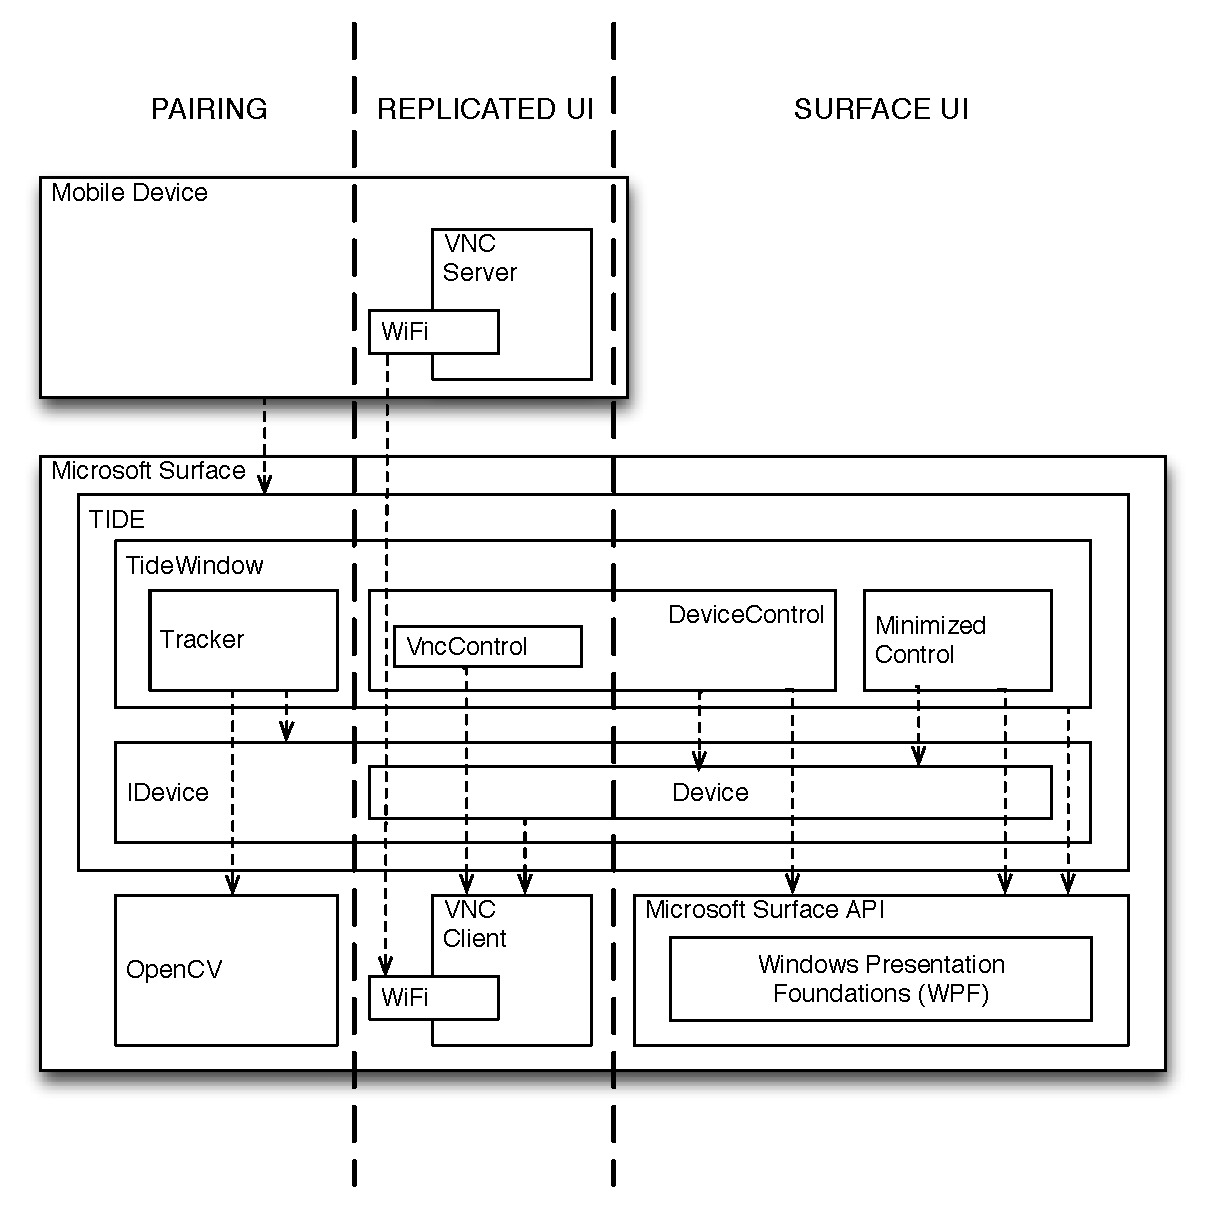
\includegraphics[width=0.8\textwidth]{images/overview}
    \caption{TIDE overview.}
    \label{fig:overview}
\end{figure}

\begin{figure}[h!]
  \centering
    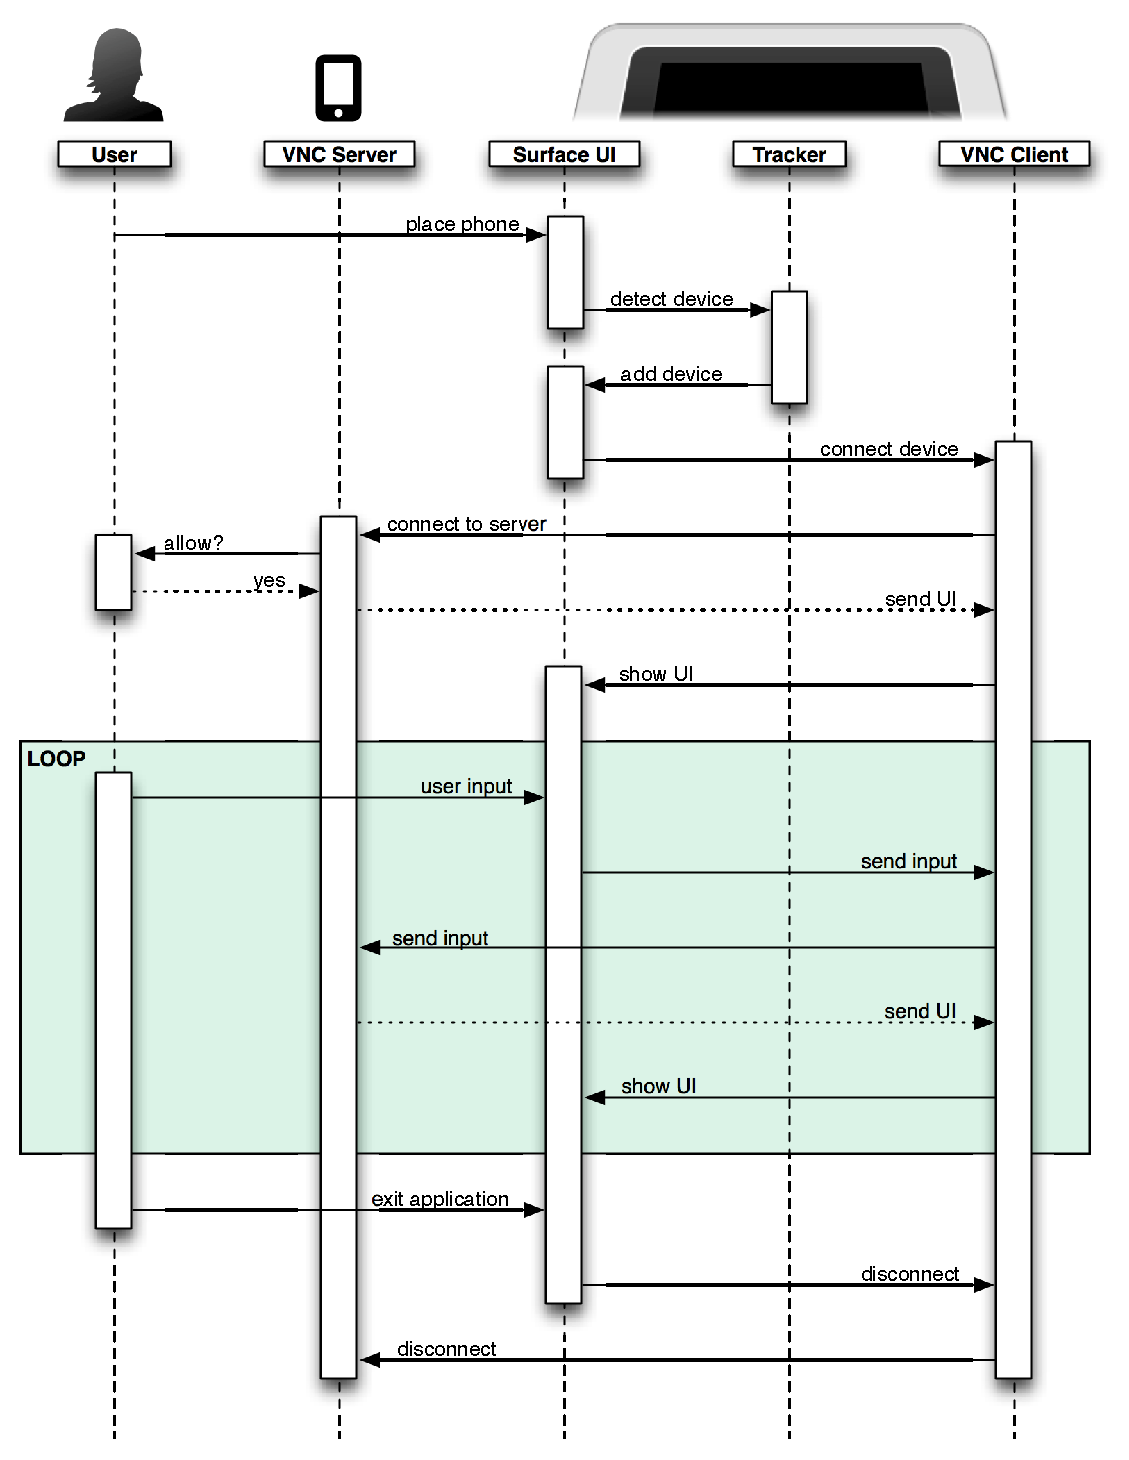
\includegraphics[width=0.8\textwidth]{images/sequenceOverview}
    \caption{TIDE overview.}
    \label{fig:sequenceOverview}
\end{figure}

%%%%%%%%%%%%%%
%% PAIRING %%
%%%%%%%%%%%%%%
\section{Pairing}
\label{sec:pairing}

The pairing procedure requires that both devices are connected to the local network.
In the case of the smartphone, this connection is very likely wireless.
Moreover, a VNC server instance should be up and running on the smartphone, for the system to function.

To achieve successful pairing, the following steps must be completed:
(1) a \emph{trigger} starts the procedure,
(2) \emph{discovery} allows the smartphone's local IP address to be made available to the tabletop and
(3) the \emph{connection} is established, given that the user explicitly authorizes it.

\subsection{Trigger}

To start the pairing procedure, a trigger must be used.
In TIDE, this trigger is provided by the detection of a smartphone object lying on the tabletop.

Interactive displays that are based on computer-vision technologies function by seeing the shape of the objects that come in contact with the surface.
That implies that not only are fingers seen, but also other objects such as books, cups, or cell phones.
The MS is an example of a tabletop that was designed for integrating with physical objects.
This strategy is based on the use of visual markers
[EXPLAIN MS VISUAL TAGS STRTATEGY HERE]

However, the MS camera-based system is able to see all contact shapes, as long as they reflect infra-red light.
The display's visual input can be captured and analyzed with computer vision algorithms such as the ones provided by OpenCV, and specific shapes can be recognized.
This strategy was used in the TIDE implementation, to detect specific smartphones, and trigger the procedure.
The details of the smartphone detection steps are explained in section~\ref{sec:tracking}.

The reason for using shape recognition instead of the MS tag recognition system is to remove as many constraints as possible, to make the system accessible to all, whatever the context.
Using visual tags would imply that the system be usable only by users that had applied a visual tag to the smartphone.

\subsection{Discovery}

The smartphone's local IP address must somehow be made available to the TIDE application, in order to establish the connection.

There is one easy solution to this problem, which is having the user enter the IP address in a dialog window on the tabletop, but this approach has serious limitations.
Finding out what the IP address is not obvious for most users, it requires digging into the networking settings of the phone.
In any case, it is a process of several steps.
Moreover, entering the address on the tabletop takes time and can lead to mistakes.
IP addresses are numeral strings of typically more then 10 digits, which makes them cumbersome to remember and type.

An easier solution is to automatize the discovery process, using networking protocols such as UPnP and Bonjour, based on Zeroconf.
[HOW MUCH SHOULD I EXPLAIN HERE??]
\\
\linebreak
Seeing that the focus of this work lies elsewhere, 
%is not to contribute within this area,
 and for reasons of time constraints, it was decided not to implement the discovery protocol.
The system currently functions with IP addresses hardcoded into the TIDE implementation on the MS, to serve the purpose of the present proof-of-concept.

\subsection{Connection}

To protect the user's privacy, the connection needs explicit authorization.
This is handled by a dialog that appears on the tabletop, described further in section~\ref{sec:surfaceui}.

The connection is otherwise handled by the VNC components on tabletop and smartphone, whose implementation details are presented in section~\ref{sec:replicatedui}.

%%%%%%%%%%%%%%
%% TRACKING %%
%%%%%%%%%%%%%%
\section{Tracking}
\label{sec:tracking}

\begin{figure}[htbp]
  \centering
    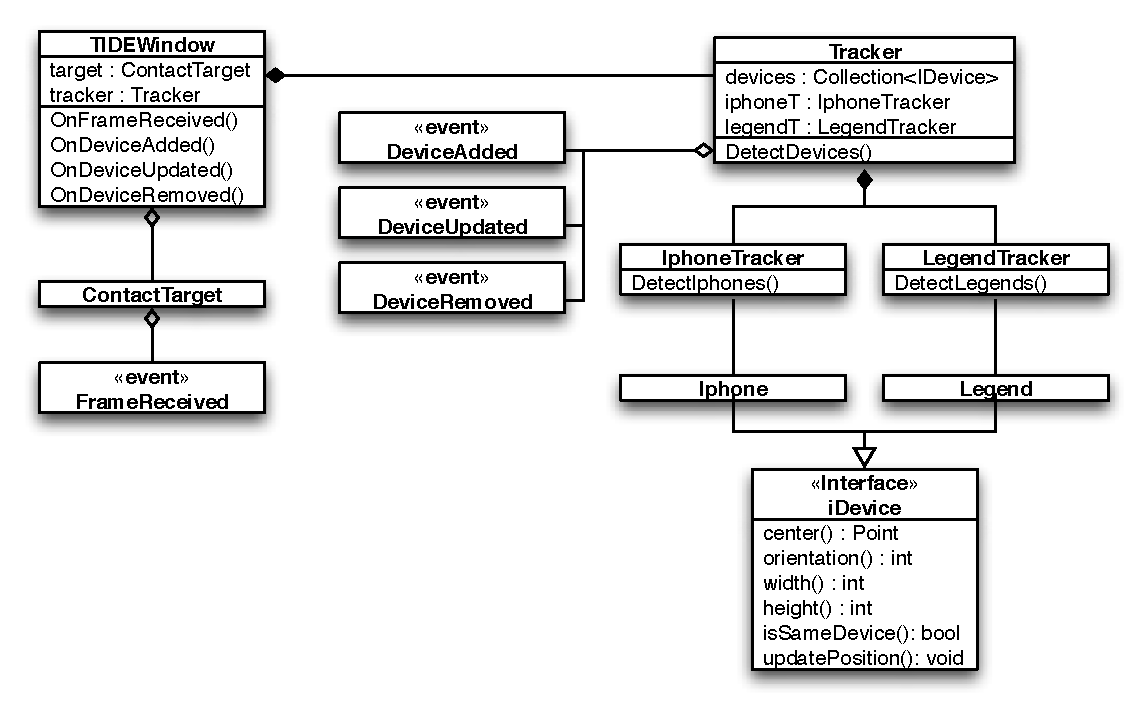
\includegraphics[width=1\textwidth]{images/trackingDiagram}
    \caption{Tracking overview.}
    \label{fig:trackingDiagram}
\end{figure}

The MS computer vision is based on infrared light that is projected towards the interactive display, and reflected by the objects that are in contact with it.
The reflection is captured by multiple cameras, and processed for system use.
By using OpenCV, it is possible to analyze the captured images to detect specific shapes and interpret the nature of the object on the table.

Figure~\ref{fig:trackingDiagram} shows the implementation of a mechanism that allows TIDE to detect specific smartphones, and track their whereabouts on the surface during application sessions.
The core layer of the Surface SDK provides the \texttt{ContactTarget} class, which raises the \texttt{FrameReceived} event for each available frame of visual input.
Figure~\ref{fig:msRaw} shows the raw MS input for both tested smartphones.
The features that allow TIDE to detect the iPhone 4 are the Apple logo and the camera point in the back of the casing.
For the HTC Legend, the system looks for the larger silver rectangle formed by the aluminum casing.

Two things can be remarked on.
First, black casing areas do not reflect infrared light, which is a basic, yet serious limitation, given that certain models of smartphones could be invisible to the system.
Second, detecting a phone depends on the specific features that the phone presents on its casing.
This implies that the system must take into considerations that the phone could be placed on the table face down, or wear a protective sleeve.

\begin{figure}[htbp]
  \centering
    \includegraphics[width=0.5\textwidth]{images/msRaw}
    \caption{Microsoft Surface raw visual input: (A) iPhone 4 (B) iPhone 4 after threshold processing (C) HTC Legend (D) HTC Legend after threshold processing.}
    \label{fig:msRaw}
\end{figure}

The \texttt{TIDEWindow} is an application-specific instance of a \texttt{SurfaceWindow} control provided by the Surface SDK Presentation layer. 
It represents the main application window, and comprises most of the application logic.
It sends screen captures to the \texttt{Tracker} class, that is responsible for processing the images, detecting and tracking the smartphones.
The \texttt{Tracker} keeps track of the devices by using additional tracker classes that are specific to the supported device types.
In the current implementation, the \texttt{IphoneTracker} detects \texttt{Iphone} objects, and the \texttt{LegendTracker} detects \texttt{Legend} objects.
All device types implement the \texttt{IDevice} interface, which provides properties that are used by the main \texttt{Tracker} to keep track of an updated list of current devices.
Upon device apparition, movement or removal, the \texttt{Tracker} raises relevant events, i.e.\ \texttt{DeviceAdded}, \texttt{DeviceUpdated}, \texttt{DeviceRemoved}.
The \texttt{TIDEWindow} listens for such events, and handles them accordingly.

The tracking component provides the application with the means to know when new devices are placed on the table, but also when and where they are moved, and when they are removed entirely.
The initial device detection was used in the evaluated prototype, as a trigger for pairing.

However, the tracking of smartphone devices during the application session was deactivated for the test sessions, for the following reason.
The purpose of tracking devices was to allow the use of the smartphone as a tangible user interface, a remote control for the replicated UI.
This feature was part of the initial requirements, as presented in section~\ref{sec:requirements}, but were left out of the final design, the reasons of which were explained in section~\ref{sec:design}.



%%%%%%%%%%%%%%%%
%% REPLICATION %%
%%%%%%%%%%%%%%%%
\section{Replicated UI}
\label{sec:replicatedui}

 (I/O approach)
- technology issues (slow Veency)

The UI replication is based on the VNC protocol \citep{Richardson:1998:vnc}.

Third-party applications were used on the smartphones, that required rooting the devices.

%%%%%%%%%%%%%%
%% SURFACE %%
%%%%%%%%%%%%%%
\section{Surface UI}
\label{sec:surfaceui}

\begin{figure}[htb]
  \centering
    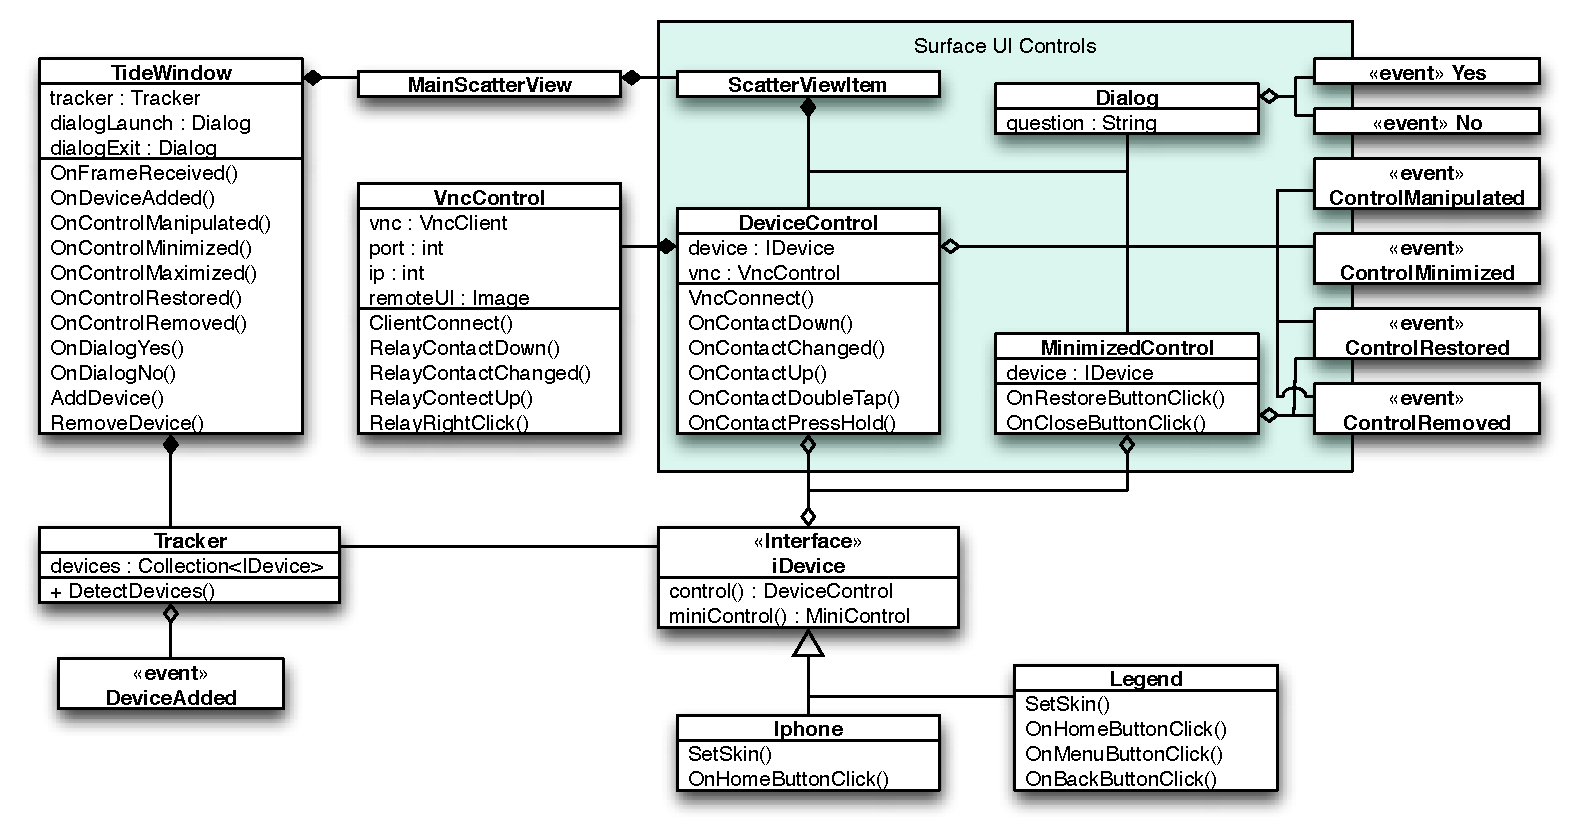
\includegraphics[width=1\textwidth]{images/surfaceDiagram}
    \caption{Surface UI overview.}
    \label{fig:surfaceDiagram}
\end{figure}


\subsection{}

we added MAXIMIZE:
Similarly when enlarged above a certain size, it is maximized to a fullscreen mode. To escape the fullscreen mode, buttons are implemented in the corners of the tabletop.






%%%%%%%%%%%%%%%%%%
%%% EVALUATION %%%
%%%%%%%%%%%%%%%%%%

\chapter{Evaluation}
\label{evaluation}

This chapter presents an evaluation of the solution designed in chapter~\ref{design}, by way of a usability study of the TIDE prototype.
The evaluation focuses on three system aspects: learnability, ease of use and usefulness.

The methods used are based on Designing Interactive Systems by
\cite{Benyon:2010}, and described in section~\ref{sec:methods}.
The evaluation results are presented in section~\ref{sec:results}.

\section{Parameters}
\label{sec:parameters}

To demonstrate that the solution proposed is valid,
this evaluation shows that TIDE allows spontaneous user interaction, and that it is a useful application.
The evaluated parameters are the system's learnability and ease of use, that are major aspects of usability; and the system's usefulness.

\begin{description}
\item[Learnability] is the capability of a software product to enable the user to learn how to use it.
%It is evaluated by engaging end users in an exploratory interaction with the system, and assessing whether this is sufficient for users to learn how to use it.

\item[Ease of use] is the self-perceived level of effort that the use of a software product requires of the user.

\item[Usefulness] is the quality of being useful, and a requirement for user satisfaction.
%It is evaluated here by asking end users to assess whether they would use the application in specific situations.

\end{description}

\subsection{Variables}

The six \emph{interaction primitives} that were defined in section~\ref{sec:strategies} are independent variables.
They are the application features that are implemented by TIDE, and the minimum set of features to allow a successful user interaction.
However, only five primitives were evaluated: \emph{dragging, rotating, resizing, minimizing and closing}.
The sixth primitive, \emph{hiding}, was removed, due to user feedback from the design process that showed it was similar, if not interchangeable, with minimizing.
\\
\linebreak
The interaction techniques that were implemented as a result of the design decisions from section~\ref{sec:design} are dependent variables.
The goal of this evaluation is to discover which of these interaction techniques are intuitive to the user and which ones the user prefers. 

%Another dependent variable is the usefulness of the system, assessed by end-users during this evaluation.

\section{Methods}
\label{sec:methods}

Given the strong focus of the present work on user interaction, it was decided to use participant-based methods to evaluate the system.
A usability study involving end-users was designed, that regrouped the selected methods in one experiment session.

\begin{description}

\item[Discovery]

To evaluate learnability, users are engaged in discovering the system on their own.
With no prior knowledge of the application, participants are given three minutes to \emph{learn by doing}, i.e.\ explore the system without exterior help.
Qualified data is gathered to evaluate how much of the system the users were able to learn.

\item[Guided test]

To evaluate ease of use, a semi-controlled experiment is designed.
Participants are asked to perform specific tasks using the system.
Detailed instructions are given to the user during the test.
These instructions mention only the independent variables, and the behavior of the user provides data to evaluate the dependent variables.
In the present case, the instructions only address the interaction primitives, and it is up to the user to choose between the available interaction techniques.
Qualified data is gathered to evaluate the dependent variables.

\item[Questionnaire]

A questionnaire is used to gather data that supports the evaluation of all three parameters.
Participants are asked to assess the learnability, ease of use and usefulness of the system by answering carefully designed questions.

\end{description}


\section{Experiment}
\label{sec:experiment}

In order to generate qualified data, a user experiment was designed and conducted.
Figure~\ref{fig:andrea} shows a participant during an experiment session.

\subsection{Participants}

Thirteen participants aged between 25 and 40 were recruited on a voluntary basis.
Five out of the thirteen had no technical background, and three out of those five were female participants.
All were regular smartphone users.

\begin{figure}[htb]
  \centering
    \includegraphics[width=1\textwidth]{images/tideandrea}
    \caption{A volunteer using the TIDE prototype.}
    \label{fig:andrea}
\end{figure}

\subsection{Apparatus}

The experiment sessions were carried out at the PITLab (Pervasive Interaction Technology) at the IT University of Copenhagen.
The TIDE prototype was installed on the Microsoft Surface tabletop computer, and used in combination with an iPhone 4 and a HTC Legend smartphone, both equipped with third-party VNC applications.
A additional desktop computer was available for filling out online evaluation forms.

\subsection{Procedure}

A session lasts 30 minutes, and involves a participant and the designer.
The session is structured by an experiment script, included in appendix~\ref{app:evalscript}, that is read by the designer to the user.

First, the participant is introduced to the following things:
\begin{itemize}
\item the structure of the session (a discovery phase, a guided test and a questionnaire),
\item the devices (Microsoft Surface, iPhone and HTC Legend);
\item the TIDE prototype:
	\begin{itemize}
	\item the pairing procedure,
	\item the lack of responsiveness of the replicated UI,
	\item the difference between the replicated UI and the surface UI;
	\end{itemize}
\item the fact that only the system is under test, not the participant.
\end{itemize}

The participant is then taken through the following phases: discovery, guided test and questionnaire.

\subsubsection{Discovering TIDE}

The participant has been shown how to pair the phone to the Microsoft Surface.
S/he is given three minutes to freely explore the application features of the application.
At the end of this discovery phase, the designer fills out the evaluation form \emph{Tide-EF1}, included in appendix~\ref{app:evalforms}, where he records for each of the interaction primitives, which of the interaction techniques the user discovered.

\subsubsection{Testing TIDE}

In order for the participant to be able to use TIDE to its full potential, s/he is taught all the available interaction techniques before the beginning of the guided test.

The test consists of two small scenarios, that require of the participant that he performs specific tasks with the application.
The first scenario involves the user and the designer playing a game of tic-tac-toe, and the second one involves the user looking up a location on Google Maps and showing it to the designer.
The tasks are explained, and detailed instructions are given to the user during the test, but for each instruction, it is up to the user to decide which interaction technique to use.
For example, the user is told to minimize the window, but not \emph{how} to activate the command.

This test allows the user to engage several times with all the interaction primitives, each time requiring that s/he chooses a technique of choice.
For example, a given user will prefer to drag a window using two hands, while another one will rather use a single finger.

The evaluation data is gathered via the questionnaire filled out during the next phase.

\subsubsection{Answering questions about TIDE}

The participant is asked to fill out a questionnaire, the evaluation form \emph{Tide-EF2}, included in appendix~\ref{app:evalforms}.
The user is asked to express an opinion about the following things:
\begin{itemize}
\item which interaction techniques are his/her favorites?
\item is the application easy to learn, easy to use, useful?
\item what is best/worst/missing in the application?
\item in which situations would the application be useful? 
\end{itemize}

%\subsection{Data}

The evaluation data was gathered via the aforementioned forms, then converted to excel files to be processed.
% as well as application logging.
The data was processed manually, analyzed, and results were derived.
%Additional data was generated through runtime logging during the application sessions.
%The logging data was not used to derive conclusive results, but to confirm the findings presented hereunder. 

\clearpage
\section{Results}
\label{sec:results}

Qualified data was generated via the previously mentioned forms \emph{Tide-EF1} and \emph{Tide-EF2}, included in appendix~\ref{app:evalforms}.
The forms were converted to excel files and processed manually.
The following results were derived from the analysis of the data.
They revealed that the system shows good learnability, ease of use and usefulness.
%These three system aspects were assessed by end users at the end of the experiment sessions.
\\
\linebreak
To get a general assessment of the application, the following 5-level Likert scale was used:
\begin{tightlists}
\begin{description}
\item[5] Strongly agree
\item[4] Agree
\item[3] Neither agree nor disagree
\item[2] Disagree
\item[1] Strongly disagree
\end{description}
\end{tightlists}
The answers are presented in figure~\ref{fig:evalagree}, where colored cells contain mean values above 4.
They confirm that the majority of the participants found the application easy to learn, easy to use and useful in context.

\begin{figure}[htb]
  \centering
    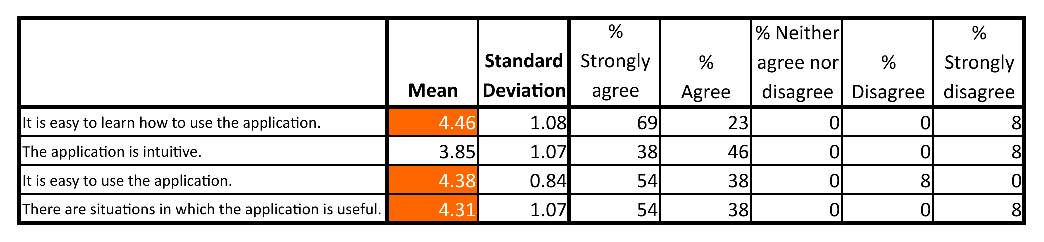
\includegraphics[width=1\textwidth]{images/evalagree}
    \caption{End users' assessment of the system's learnability, ease of use and usefulness.}
    \label{fig:evalagree}
\end{figure}

For each of the evaluated parameters, further results were derived from the experiment data.

\subsection{Learnability}

All participants were able to discover at least one technique to perform each of the necessary primitives to a successful interaction with the system.
In other words, all participants could find out on their own and within three minutes how to drag, rotate, resize, minimize and close the main application window on the tabletop.

It can thus be concluded that the system implements interaction techniques that comes naturally to most users.
Figure~\ref{fig:evaldisco} shows which specific techniques were discovered by the participants. The colored cells contain values above 50\%.
%The experiment here could have been made more interesting:
%- differentiation of ways to drag the window around (1 or 2 fingers?) 

\begin{figure}[htb]
  \centering
    \includegraphics[width=0.7\textwidth]{images/evaldisco}
    \caption{Interaction techniques that were discovered by the end users.}
    \label{fig:evaldisco}
\end{figure}

The first thing that can be remarked upon is that, although all the basic shape manipulation techniques were easily discovered, the two-handed rotating and resizing gestures scored higher than their single-handed counterpart.
This points towards the fact that it is more intuitive to perform these gestures with both hands.

Given that all participants could somehow resize the window, 85\% logically found out that they could use it to minimize it as well.
In most cases, the user stumbled upon this feature by accident, while exploring the resizing feature.
This is an example of how design can enable the user to \emph{learn by doing}.

Only 46\% of the users found out that the window could be minimized by being dragged to the edge, and none discovered the possibility of closing the window by bringing it to a corner.
These techniques were implemented because of their success among end users during the design sessions based on low-fidelity prototypes.
They were expected to be easy to discover because of their consistency with how people would interact with a document on a normal table.
However, it seems that this success was prompted by the fact that  the prototypes were actual pieces of paper, which could only be minimized/hidden/closed by being physically put away.

Similarly, none discovered that the window could be minimized by tapping it with the whole hand, even though the gesture was thought to be natural due to its resemblance to the action of hiding a document on a normal table.
It can be remarked that this gesture is not used on common devices such as smartphones or personal computers.
It is a gesture that requires a lot of space and is therefore specific to large interactive surfaces, and thus not part of the common IT knowledge of most users.

69\% of the participants found out about the double tap, which is a large amount, considering the fact that the feature is hidden, i.e.\ it can not be discovered by accident while exploring the manipulation possibilities, but has to be explicitly attempted.
It shows that, as opposed to the whole hand tap, the double tap is part of the common IT knowledge.

Pressing and holding on the window to close it is also a hidden feature, and it was discovered by none.
However, the results concerning the primitive \emph{closing} are not considered conclusive, due to the fact that users did not attempt to discover different ways to close the application during the exploratory phase, but only performed it once to terminate the session.

\subsection{Ease of use}

To determine which interaction techniques were the most efficient, participants were asked to select their favorites.
The answers are presented in figure~\ref{fig:evalfavor}, where colored cells contain values above 50\%.
This study only addresses the primitives for which multiple techniques were implemented.\footnote{Two techniques were not included in the study due to a human mistake: rotating with 1 finger and closing with press and hold.}
Participants were not limited to select one technique per primitive.

\begin{figure}[htb]
  \centering
    \includegraphics[width=0.7\textwidth]{images/evalfavor}
    \caption{End users' favorite interaction techniques.}
    \label{fig:evalfavor}
\end{figure}

It is interesting to see that users preferred to resize and rotate by using a two-handed gesture, even though it could be done single-handedly.
An explanation might be that the two-handed gesture seems to provide more control to the user, especially when s/he has little experience with touch shape manipulation on large surfaces.
%Especially since using two hands allow the user to grab the shape at both its extremities
%This is especially true given that most users had little or no prior experience with large touch screens.

To minimize, the favored techniques were double tap and the whole hand tap.
Resizing the window down to minimize it was only favored by 8\% of the users, even though it was the most easily discovered technique, whereas using a whole hand tap could not be discovered, but ended up among the most appreciated ones.
This shows that familiar and efficient features are not necessarily the same, and that both are needed.
The familiar gestures make the system easy to learn, while the efficient ones, such as the double tap or the whole hand tap, make it easy to use.

The gestures that involved dragging the window to an edge or corner of the tabletop did not score as high as expected among the participants.
The hypothesis that such gestures would be appreciated because of their consistency with normal table interaction, i.e.\ their similarity with the action of putting a document away, was not confirmed.
The first explanation that comes to mind is that a dragging gesture requires more time and space to be performed than, say, a double tap, which is quicker and can be done on the spot.


\subsection{Usefulness}

The participants expressed the opinion that the application would be useful in specific situations.
As part of the questionnaire, they were asked which activities they would consider using the system for, and in which context.
The answers are presented in figure~\ref{fig:evalcontext}, where colored cells contain values above 50\%.

\begin{figure}[htb]
  \centering
    \includegraphics[width=1\textwidth]{images/evalcontext}
    \caption{The contexts in which the application is useful.}
    \label{fig:evalcontext}
\end{figure}

The participants were presented with a list of 7 activities that could be performed on a smartphone.
For each of those activities, the users were asked first if they would use their smartphone to do them, then in which context they would consider using the application instead.
The contexts suggested were: alone in a private space, alone in a public space, together with friends or colleagues.

The results show that whether a user would choose the application or not depends mostly on privacy and trust.

The first realization is that the system is not a proper platform for activities that involve private data.
There are two activities that most users do on smartphones, but very few would do on a tabletop, whatever the context: reading and writing emails or sms messages.
Both activities involve viewing text that would potentially contain personal conversations.
It is therefore natural, that users would not want to view this data on the large open display of a tabletop.

The second realization is that there are indeed a series of activities for which the system is suitable.
They are: browsing the internet, looking at pictures, playing games and looking at a map.
However, most users would only use the application for these activities in a \emph{trusted} context, i.e.\ in a private space, or together with trusted acquaintances.
In a public context, the only activity that a majority of users would still consider doing with the system is looking up a location on a map.
Again, the explanation to this can probably be found in the fact that tabletops are very public devices, in the sense that they can be seen by any person in range.
Unlike smartphones, laptops, or even desktops, whose screen can be rotated more or less freely, tabletop displays are there for the world to see.
Thus, users are reticent to use them in public, even for semi-private occupations such as browsing the internet or playing games.

Last but not least is the realization that the system has most potential for the activity of reading documents.
It is the only activity that only a minority of users (31\%) would do on a smartphone, which confirms the hypothesis that smartphone screens are too small for this type of graphically intense data.
62\% of the participants would consider using the application for reading documents, though only in a trusted context.
Thus, the system seems to address a real need.



















\chapter{Discussion}
\label{discussion}

Implementing same functionality with several parallel interaction techniques is a good choice because it will augment the number of situations in which a user will obtain the desired effect intuitively on his first try, without referring to any manual.

%%%

However, due to limitations implemented by the manufacturers, installing the VNC applications required rooting the devices.
Rooting a smartphone is a procedure that allows the user to obtain full access rights on the system, though with the implication that the device warranty becomes void.
Thus, it cannot be expected of users that they will perform this procedure, and this approach would be problematic in a real-world scenario.
However, this setup was satisfying for the purpose of the proof-of-concept.

[VNC IS NOT ADAPTED TO THIS SITUATION; IT IS TOO SLOW]


\chapter{Conclusion}
\label{conclusion}

%\cleardoublepage
%\chapter*{Bibliography}
%\addcontentsline{toc}{chapter}{Bibliography}

\bibliographystyle{plainnat} %abbrv,ieeetr
\bibliography{../references}

%\cleardoublepage
%\part*{Appendices}
%\addcontentsline{toc}{part}{Appendices}

\settocdepth{chapter}

\part*{Appendices}
\addcontentsline{toc}{part}{Appendices}

\appendix
\chapter{TIDE video and code}
\label{video}

A short video describing the system, as well as the TIDE source code, are available with the project description on the PITLab's website:\\
\linebreak
\texttt{http://www.itu.dk/pit/?n=Projects.Devicecomposition}



\documentclass[11pt]{amsart}
\usepackage{geometry}                % See geometry.pdf to learn the layout options. There are lots.
\geometry{letterpaper}                   % ... or a4paper or a5paper or ... 
%\geometry{landscape}                % Activate for for rotated page geometry
%\usepackage[parfill]{parskip}    % Activate to begin paragraphs with an empty line rather than an indent
\usepackage{graphicx}
\usepackage{amssymb}
\usepackage{epstopdf}
\DeclareGraphicsRule{.tif}{png}{.png}{`convert #1 `dirname #1`/`basename #1 .tif`.png}

\title{OpenTable - Scenarios}
\author{Leo Sicard}
%\date{}               % Activate to display a given date or no date

\begin{document}
\maketitle

\section{The Coffee Shop}

Alice is supposed to meet her friend Bob in a Coffee Shop.
She arrives early, and chooses to sit at one of the interactive tables.
After ordering a drink via the tabletop, she takes her phone out of her purse (turns on the WIFI) and places it on the table.
A popup dialog window appears next to her smartphone, asking Alice to confirm the establishment of a UI transfer.
Alice accepts, and her phone's screen appears on the larger surface, seemingly attached to her physical device.
She resizes the UI to her convenience, and moves it closer to her by sliding her phone on the surface.
Alice is thus able to use her smartphone's applications on the larger surface while waiting for Bob. She writes and sends an email, and browses the internet.

When Bob arrives, Alice minimizes her screen next to her phone, but keeps the connection active.
Bob orders a drink and they start catching up.
Bob has just returned from a vacation and he has pictures on his smartphone that he wishes to show Alice.
He connects his phone to the table as Alice had done, so that they can both look at the pictures on the larger screen of the table. When done, Bob disconnects his phone by simply lifting it off the table.
After a while, they decide to go watch a movie.
Alice restores her phone's UI on the table and opens a browser in order to access the program of the closest cinema.

\section{The Meeting}

Jim, Jack and Jill are having a meeting about the development of a software product.
They are sitting around an interactive table, with different artefacts, including paper, pens, computing devices and coffee cups.
Jill is directing the meeting, she has her smartphone placed on and connected to the table, its screen extended to a portion of the surface.
On the screen is a text document presenting the agenda, Jack and Jim are also able to easily refer to the different points of the agenda.

Jack's task is to show and explain a diagram to the others.
He switches on his tablet computer, opens said diagram, and places the tablet on the table for the others to see.
Jack connects his device to the surface, thus allowing the tablet's screen to be extended to the surface.
Jack attaches the UI to the table, allowing him to remove the tablet.
He uses simple touch to resize and rotate the window, and presents the diagram to his colleagues.
When done, Jack switches off his tablet computer, which has the effect of interrupting the connection to the table and instantly closing the diagram window.


\section{The Office}

It is monday morning and Bill arrives at his office.
His desk is an interactive table.
On it are a laptop computer, stacks of papers, books, pens, an empty cup and a lamp.
Bill powers on the tabletop and laptop, and places his smartphone on the table.
Bill's smartphone is known to the tabletop, and therefore the UI connection is automatically established in dual view mode, allowing Bill to drag widgets out of his smartphone.
Bill places its calender up in one corner, together with its Skype widget.
After reading through his mail on the laptop computer, Bill starts writing an answer, for which he needs to refer to a document that is stored on the smartphone.
Bill switches to a mirrored display mode for his phone, causing its screen to appear on the table, attached to the device.
By sliding the phone, he moves the display to a convenient location.
Suddenly the phone rings.
Bill attaches all applications and UI display to the table, allowing him to pick up the phone without losing his open document nor widgets.






\end{document}  

\chapter{Design experiment}

\tightlists

\section{Experiment script}
\label{app:study}

\subsection{Introduction}
``You are here to participate in a short experiment where you will assist in the design of an application called TIDE.
The experiment will last about 30 minutes and will be recorded, both as audio and video.
I will give you instructions by reading from this script.
After an introduction you will be able to ask questions, then we will start the experiment.

First, let me introduce TIDE.
TIDE is an application that connects a smartphone (iPhone) with a tabletop computer (Microsoft Surface).
It allows you to interact with your phone on a larger screen, by transferring the display of your phone to a window on the screen of the interactive surface.
Do you understand the basic concept of the application?

During this experiment, I will ask you to perform a task using the application.
This will lead you to perform a number of actions that use the basic features of TIDE.
For each action, there will be 3 steps:

\begin{itemize}
\item{First, I will explain the action, and show you its effect on this screen}
\item{Second, I will ask you to describe to me how you would suggest performing this action with the user interface of TIDE.}
\item{Third, I will give you 3 suggestions of how to perform the action, and ask you to order them according to your preference.}
\end{itemize}

This experiment is based on prototypes, which means that we will use the available paper representations, in order to describe the user interface of TIDE.
There are iPhone screenshots and different types of buttons and controls.
Paper, pen and scissors are available for building your own prototypes if necessary.
You are welcome to draw on the prototypes as needed.
We will also use the iPhone, the MS Surface, and of course verbal communication.
\hfill\\
This iPhone screenshot printout is a representation of the main window of the TIDE application.
The idea is that you can interact with this window in exactly the same way as you would interact with your phone's screen.
For example, by tapping the Photos icon, you would launch the Photos application, and if you are viewing a picture, by performing a two finger pinching gesture, you could zoom on the picture.
At the same time, we need a way to manipulate the window, and that is what the focus of this experiment
\hfill\\
Do you have any questions concerning the general course of the experiment?
\hfill\\
Let us begin.
Your general task is to write an email to a friend using your iPhone and the TIDE application on the Microsoft Surface.
We will talk about 7 basic actions.''

\subsubsection{Example: Pairing}
\hfill\\
This first action is only an example, meaning that I will go through all the steps.
The action is called pairing.
\hfill\\
\hfill\\
\emph{Scenario:}
In order to use TIDE, I have to pair my iPhone with the Surface and launch the TIDE application.
Here is a visual representation of the effect of this application (the designer shows a PowerPoint animation that describes the command).
\hfill\\
\hfill\\
\emph{Suggestion:}\\
I asked my friend Juan, and his suggestion was to launch TIDE on the iPhone, then search for available surface computers within the application,  and connect to the Surface.
\hfill\\
\hfill\\
\emph{Selection:}
\begin{description}
\item[A]{The application launches automatically when the smartphone is placed on the surface, and a dialog window appears on the smartphone, offering the user to establish the connection.}
\item[B]{The application launches automatically when the smartphone is placed on the surface, and 2 dialog windows appear, first on the surface, then on the smartphone, offering the user to establish the connection.}
\item[C]{The application launches automatically when the smartphone is close enough to the surface, and a dialog window appears on the surface, offering the user to establish the connection.}
\end{description}

Juans order of preference was B, A, C.
What about you?
\hfill\\
\hfill\\
There are 6 actions left, and I will now show you visual representations for each of those actions (the designer shows a PowerPoint animation that describes the commands).

\subsection{Experiment}

%%%%%%%%%%%%%%%%%%
% DRAGGING

\subsubsection{Dragging}
\emph{Scenario:}
Your iPhone screen is now active on the surface, and you need to move it closer to yourself. Therefore, you drag the window across the surface.
\hfill\\
\hfill\\
\emph{Suggestion}
\hfill\\
\hfill\\
\emph{Selection (group 1)}
\begin{description}
\item[A]{By performing a one finger dragging gesture on a specific action tab. (1)}
\item[B]{By performing a one finger dragging gesture on the action bar. (2)}
\item[C]{By tapping a tab to render the window inactive, then performing a one finger dragging gesture anywhere on the window. (3)}
\end{description}
\hfill\\
\emph{Selection (group 2)}
\begin{description}
\item[A]{By performing a one finger dragging gesture on the active border of the window. (4)}
\item[B]{By performing a one finger dragging gesture on the active border (excl. corners) of the window. (5)}
\item[C]{By holding a finger on a specific tab, and using another finger to tap a destination target to move the window to. (6)}
\end{description}

%%%%%%%%%%%%%%%%%%
% ROTATING

\subsubsection{Rotating}
\emph{Scenario:}
the application window is not oriented correctly, so you need to rotate it to the correct orientation. 
\hfill\\
\hfill\\
\emph{Suggestion}
\hfill\\
\hfill\\
\emph{Selection (group 1)}
\begin{description}
\item[A]{By performing a two finger touch rotating gesture on the action bar. (2)}
\item[B]{By tapping a tab to render the window inactive, then performing a two finger touch rotating gesture anywhere on the window. (3)}
\item[C]{By performing a two finger touch rotating gesture on the active border. (4)}
\end{description}
\hfill\\
\emph{Selection (group 2)}
\begin{description}
\item[A]{By performing a two finger touch rotating gesture on the active border. (5)}
\item[B]{By performing a one finger dragging gesture on a corner of the window. (6)}
\item[C]{By performing a two finger touch rotating gesture with one finger placed on a specific tab, and the other finger anywhere on the window. (1)}
\end{description}

%%%%%%%%%%%%%%%%%%
% RESIZING

\subsubsection{Resizing}

\emph{Scenario:}
Now you open the Safari App by taping on the correct icon, but the window is too small for you to type an email, so you resize it to make it bigger.
\hfill\\
\hfill\\
\emph{Suggestion}
\hfill\\
\hfill\\
\emph{Selection (group 1)}
\begin{description}
\item[A]{By tapping a tab to render the window inactive, then performing a two finger pinching gesture anywhere on the window. (3)}
\item[B]{By performing a two finger pinching gesture on the active border. (4)}
\item[C]{By performing a one finger dragging gesture on an active corner. (5)}
\end{description}
\hfill\\
\emph{Selection (group 2)}
\begin{description}
\item[A]{By pulling the window apart with both hands. (6)}
\item[B]{By performing a one finger dragging gesture on a specific tab. (1)}
\item[C]{By performing a two finger pinching gesture on the action bar. (2)}
\end{description}


%%%%%%%%%%%%%%%%%%
% MINIMIZING

\subsubsection{Minimizing}

\emph{Scenario:}
Before you start writing your email, you want to verify some facts in a document.
You decide to minimize the TIDE application to make room for the paper, and to be able to restore the window to its previous state quickly.
\hfill\\
\hfill\\
\emph{Suggestion}
\hfill\\
\hfill\\
\emph{Selection (group 1)}
\begin{description}
\item[A]{By double tapping the active border. (4)}
\item[B]{By using Resizing on an active corner to reduce the window until it snaps to icon shape. (5)}
\item[C]{By dragging the window to the bottom of the surface. (6)}
\end{description}
\hfill\\
\emph{Selection (group 2)}
\begin{description}
\item[A]{By tapping a specific tab. (1)}
\item[B]{By double tapping the action bar. (2)}
\item[C]{By tapping a tab to render the window inactive, then performing a specific gesture anywhere on the window. (3)}
\end{description}

%%%%%%%%%%%%%%%%%%
% HIDING

\subsubsection{Hiding}

\emph{Scenario:}
Later, you are writing another email of a personal nature, and one colleague is approaching. You wish to quickly and temporarily hide what you are doing.
\hfill\\
\hfill\\
\emph{Suggestion}
\hfill\\
\hfill\\
\emph{Selection (group 1)}
\begin{description}
\item[A]{By double tapping an active corner. (5)}
\item[B]{By placing and holding a hand on the window. (6)}
\item[C]{By tapping a specific tab. (1)}
\end{description}
\hfill\\
\emph{Selection (group 2)}
\begin{description}
\item[A]{By performing a specific gesture on the action bar. (2)}
\item[B]{By tapping a tab to render the window inactive. (3)}
\item[C]{By double tapping the active border. (4)}
\end{description}


%%%%%%%%%%%%%%%%%%
% EXITING

\subsubsection{Closing}

\emph{Scenario:}
Finally, you are finished and want to leave. You close the TIDE application.
\hfill\\
\hfill\\
\emph{Suggestion}
\hfill\\
\hfill\\
\emph{Selection (group 1)}
\begin{description}
\item[A]{By dragging the window to a specific location on the surface. (6)}
\item[B]{By tapping a specific tab. (1)}
\item[C]{By performing a specific gesture on the action bar. (2)}
\end{description}
\hfill\\
\emph{Selection (group 2)}
\begin{description}
\item[A]{By tapping a tab to render the window inactive, then performing a specific gesture on the window. (3)}
\item[B]{By using Resizing on the active border to Minimize, then tapping a specific tab. (4)}
\item[C]{By using Resizing on an active corner to Minimize, then tapping a specific tab. (5)}
\end{description}



\chapter{Design - experiment form}
\label{app:studyForm}

\begin{figure}[htb]
  \centering
    \includegraphics[width=1\textwidth]{images/studyForm}
  \caption{Form used to gather participant answers during the design experiment.}
  \label{studyScreenshot}
\end{figure}

\documentclass[11pt]{amsart}
\usepackage{geometry}                % See geometry.pdf to learn the layout options. There are lots.
\geometry{letterpaper}                   % ... or a4paper or a5paper or ... 
%\geometry{landscape}                % Activate for for rotated page geometry
%\usepackage[parfill]{parskip}    % Activate to begin paragraphs with an empty line rather than an indent
\usepackage{graphicx}
\usepackage{amssymb}
\usepackage{epstopdf}
\DeclareGraphicsRule{.tif}{png}{.png}{`convert #1 `dirname #1`/`basename #1 .tif`.png}

\title{TIDE user experiment}
\author{lnsi}
%\date{February 2012}                                           % Activate to display a given date or no date

\begin{document}
\maketitle

\emph{Introduction speech to the user:}
\\\\
``The experiment is divided in 3 parts.
First, you will learn how to use the application.
Second, I will guide you through two scenarios where you will use the application to do specific things.
Third, I will ask you to answer to a questionnaire.

The Microsoft Surface is a tabletop computer with an interactive display.
You interact with it by using finger touch, like on a smartphone.

The TIDE application allows you to connect a smartphone to the tabletop.
To do that, you only need to put the phone on the table.
An application window appears on the table screen, which resembles the phone.
You can manipulate the window, but if you touch inside, the input will be relayed to the phone.

This is a prototype, implying that the application presents some defaults.
The main issue is that there is an important lag when interacting with the phone, please be patient.
Unexpected behavior might occur, in which case I will step in to keep the experiment on track.''

\section{Discovering Tide (10 min)}

The user discovers the application and learns to use its features.
First by himself, then with the support of the designer.

\subsection{Free exploration}
 
The user has 5 minutes to freely try the prototype, understand how it works and discover its features.

\subsection{Features}

User and designer go through each command together.
For each command, the user shows which actions he knows.
If there are any unknown actions, the designer teaches them to the user.

The designer fills out the form Tide-EF1.

\section{Using Tide (10 min)}

The designer guides the user through two scenarios where the user performs various tasks using the application.
The designer tells the user what to do, but not how to do it.

\subsection{Gaming}

Scenario: user and designer are two friends in a waiting room. They play a game of tic-tac-toe to pass the time.

\begin{enumerate}
\item connect the iPhone to the tabletop
\item launch the game called 'tic tac toe'
\item start a 2 players game
\item position and resize the window to allow for 2 players to interact
\item now we play
\item exit the game
\item close the application
\end{enumerate}

\subsection{Browsing}

Scenario: user and designer are planning a surprise dinner at a restaurant for the birthday of a friend. The user uses the application to go online and find the address of a restaurant, then to find how to go from the university to the restaurant.
When the friend is close, the user should hide what he is doing.

\begin{enumerate}
\item connect the HTC Legend to the tabletop
\item adjust the position and size of the window
\item launch the app called Internet
\item find the address of 'restaurant aristo'
\item minimize the window to hide what you are doing
\item restore the window
\item launch the app called Maps
\item look up the address for the restaurant
\item zoom in on the restaurant
\item find out how to walk from ITU to the restaurant
\item rotate the window to show me how to walk from ITU to the library
\item minimize the window to hide what you are doing
\item restore the window
\item return to phone home screen
\item exit application
\end{enumerate}

\section{Questionnaire (10 min)}

The user fills in the evaluation form Tide-EF2.

%teaching phase for each primitive (5):
%1) ask them to do it
%	- do they know how to do it
%	- which technique do they use?
%2) ask them if they know of other technique
%- if yes, which? show?
%- if no, tell them. show?
%
%scenario phase:
%1) browsing:
%- pair Legend
%- look up sthg online: remote UI, dragging, resizing
%- shoe me sthg: rotating
%- hide stag from someone: minimizing/hiding
%
%2) gaming (designer is opponent)
%- pair iPhone
%- launch game: remote UI
%- resize to fullscreen (maximize)
%- exit
%
%questionnaire phase: google forms?
%= straightforward user satisfaction study
%- rate the experience: usable? engaging?
%- would you use such a system?
%- how intuitive is the system?
%
%
%LOGGING (user, session, command, action, timestamp)
%
%drag, resize, rotate = using active border
%
%maximize by size enlarge
%rotate when maximized
%
%minimize by drag to edge
%minimize by double tap
%minimize by blob touch
%minimize by size reduce
%
%close by minimize
%close by corner
%close by press and hold

\end{document}

\end{document}